\documentclass[conference]{IEEEtran}
\IEEEoverridecommandlockouts
\usepackage{cite}
\usepackage{amsmath,amssymb}
\usepackage{booktabs,array,tabularx,multirow}
\usepackage{tikz}
\usepackage{url}
\usepackage[hidelinks,pdfauthor={},pdftitle={Confidence-Bounded Physical Feasibility Ranking for Neutronic Screening of QUBO-Feasible Fuel Layouts Using OpenMC}]{hyperref}
\usetikzlibrary{arrows.meta,positioning,calc}
\title{Confidence-Bounded Physical Feasibility Ranking for Neutronic Screening of QUBO-Feasible Fuel Layouts Using OpenMC}
\author{\IEEEauthorblockN{Anonymous Authors}\\
\IEEEauthorblockA{Affiliations withheld for double-blind review}}
\begin{document}
\maketitle

\begin{abstract}
Composition feasibility under a binary-quadratic objective does not establish physical acceptability, and a post-simulation rule cannot justify a unique choice when the evidence leaves candidates tied. This paper reports an evidence-audited, exploratory implementation of Confidence-Bounded Physical Feasibility Ranking (CB-PFR) on a two-dimensional multigroup C5G7-derived fuel-placement case. Four fuel positions receive exactly two mixed-oxide (MOX) and two uranium-dioxide assemblies, while five reflector positions remain fixed, producing six enumerated labels and four diagonal-reflection symmetry classes. A composition-only quadratic unconstrained binary optimization (QUBO) penalty gives every feasible label zero energy; no pre-physics optimizer or annealer was run. In the 18-run OpenMC layout campaign, a retrospective illustrative screen passes two symmetry classes and fails two, but the thresholds were selected after the runs and are not engineering limits. An additional three-seed UMMU repeatability assessment produced different results under 500 and 100 inactive-batch protocols: mean $k_{\mathrm{eff}}=1.18649321$ ($-5.68$ pcm) and between-run SD 15.57 pcm for the former, versus 1.18647358 ($-7.64$ pcm) and 0.77 pcm for the latter. The dispersion discrepancy and source-convergence diagnostics remain unresolved. The results demonstrate traceable screening and tie handling, not benchmark validation, physical optimality, calibrated confidence coverage, comparative superiority, or quantum advantage.
\end{abstract}

\begin{IEEEkeywords}
CB-PFR, C5G7 benchmark, OpenMC, QUBO, reproducible research software
\end{IEEEkeywords}

\section{Introduction}
Discrete optimization can satisfy an encoded constraint without establishing that a candidate is physically acceptable. A binary-quadratic objective distinguishes candidates only through terms it represents \cite{kochenberger2014,usmanov2024}. Reactor loading-pattern studies have used genetic algorithms, simulated annealing, hybrid schemes, and problem-specific encodings, although their objectives and reactor models differ by application \cite{chapot1999,wu2001,erdogan2003,zameer2014,sobolev2017}. More recent work combines adjoint-based physical information with evolutionary search \cite{abuzlf2025}. These studies motivate separation between the search objective and physical assessment; they are not direct performance baselines for this small enumerated case.

This paper studies CB-PFR (Confidence-Bounded Physical Feasibility Ranking) as a transparent post-simulation screening component in a research-software workflow. Its contribution is bounded: the implementation makes declared limits, uncertainty semantics, violations, and ties visible; the accompanying C5G7/OpenMC case study shows how those rules behave on recorded data. It is not a claim that CB-PFR is superior to established constraint-handling or stochastic ranking methods, nor that a scalable optimizer has been demonstrated. In particular, all six feasible layouts were enumerated; no pre-physics optimizer or annealer was run.

\section{Case Study and Methods}
\subsection{Candidate Space and Composition QUBO}
The two-dimensional model fixes five reflector positions and varies four fuel positions \(p_{00},p_{01},p_{10},p_{11}\). Each fuel position receives either MOX or UO$_2$, with exactly two of each. The six label strings are MMUU, MUMU, MUUM, UMMU, UMUM, and UUMM. Let \(y_i\in\{0,1\}\) indicate MOX at position \(i\). The composition-only penalty is
\begin{equation}
E(\mathbf y)=A\left(\sum_{i=1}^{4}y_i-2\right)^2,\qquad A>0.
\label{eq:qubo}
\end{equation}
Using \(y_i^2=y_i\), its expansion is
\begin{equation}
E(\mathbf y)=A\left(4-3\sum_i y_i+2\sum_{i<j}y_iy_j\right).
\end{equation}
Every feasible assignment has \(\sum_i y_i=2\), hence \(E=0\). This algebraic degeneracy is a limitation of the stated composition-only objective, not of QUBO in general. The study is a complete enumeration of a small design space and does not test whether a pre-physics optimizer is useful at larger scales.

\subsection{Symmetry and Neutronic Metrics}
The declared \(3\times3\) position map places the four variable fuel locations at the upper-left \(2\times2\) positions and the five reflectors elsewhere. Reflection across the main diagonal swaps \(p_{01}\) and \(p_{10}\). Thus MMUU/MUMU form class S1, MUUM is S2, UMMU is S3, and UMUM/UUMM form S4. This class reduction depends on the documented mapping and symmetric model assumptions.

OpenMC is used for multigroup neutron-transport and tally calculations \cite{romano2015}; the C5G7 MOX specification provides the benchmark context \cite{nea2003}. For the four variable fuel regions, let \(R_i\) be the assembly-integrated fission tally. The relative peaking proxy is
\begin{equation}
F=\frac{\max(R_1,R_2,R_3,R_4)}
{\frac{1}{4}\sum_{i=1}^{4}R_i}.
\label{eq:fpeak}
\end{equation}
\(F\) is dimensionless and relative. It is not absolute power, pin power, a thermal-hydraulic quantity, or an approved safety criterion. Source-distribution entropy and \(k\)-generation traces are used as descriptive diagnostics; monitoring source convergence is important in eigenvalue calculations, but no single scalar diagnostic alone certifies convergence \cite{openmcguide}.

\subsection{CB-PFR Rule}
For candidate or symmetry class \(i\) and metric \(j\), let \(\bar{x}_{ij}\) be the observed estimate and \(s_{ij}\) the supplied uncertainty summary. CB-PFR forms operational bounds
\begin{equation}
B_{ij}^{-}=\bar{x}_{ij}-z_js_{ij},\quad
B_{ij}^{+}=\bar{x}_{ij}+z_js_{ij}.
\label{eq:bounds}
\end{equation}
For declared lower and upper limits \(L_j,U_j\), violation is
\begin{equation}
v_{ij}=\max(0,L_j-B_{ij}^{-})+\max(0,B_{ij}^{+}-U_j),
\end{equation}
including only terms for limits that are declared. The normalized violation is \(V_i=\sum_j w_jv_{ij}/d_j\), where \(w_j\geq0\) and \(d_j>0\) are the metric weight and scale. These operational bounds are not calibrated confidence intervals. Missing or invalid required values fail closed.

When feasible candidates have identical substantive scores, CB-PFR reports a tie. An input-order fallback, if used for reproducible display, is not a physical preference. A separate downstream selector may apply an explicitly declared secondary score, but it does not make the composition-only pre-physics QUBO informative and is not an optimizer advantage result.

\subsection{Archived Campaigns and Exploratory Limits}
The six-layout campaign contains 18 recorded multigroup OpenMC runs: six labels across seed rounds 820000, 830000, and 840000. Each used the documented seven-group C5G7 energy structure, 7,000 total batches, 500 inactive batches, 10,000 particles per batch, and two threads. The records contain unique seeds and statepoint hashes and a common multigroup cross-section (MGXS) hash. These archive checks support traceability, but the model geometry/material mapping and spatial-tally correspondence have not been independently reviewed against the primary specification.

A separate three-seed UMMU repeatability assessment used the same total batch count (7,000) and particles per batch (10,000) under two protocols: 500 inactive batches in one archived run set and 100 inactive batches in a later run set. The 500-inactive simulations completed and their raw HDF5 audits passed, but the initial aggregation job stopped because the source-convergence report for seed 720000 was absent. The archived statepoints were subsequently inspected directly for active-batch entropy and $k$-generation traces. The later 100-inactive run set produced these reports but logged repeated warnings that fission-source sites fell outside the entropy mesh. The two protocols are therefore reported separately rather than pooled or presented as interchangeable replications.

No design-specific acceptance rule was independently approved before the six-layout campaign. Therefore, \(k_{\mathrm{eff}}\in[1.14,1.21]\), \(F_{\max}=1.35\), \(z=1\), scales \(d_k=0.01\), \(d_F=0.1\), and unit weights are explicitly retrospective illustrative settings. They exercise the software pathway only. A sweep over \(F_{\max}\in\{1.30,1.32,1.35,1.80,1.82,1.87,1.90\}\) and \(z\in\{0,1,2\}\) is sensitivity analysis, not confirmation.

\section{Results}
\subsection{Symmetry-Class Aggregation}
Table~\ref{tab:classes} summarizes class-level run results. \(s_{k,\mathrm{run}}\) is the sample standard deviation of run-level \(k_{\mathrm{eff}}\) means within each class; \(\bar{s}_{k,\mathrm{within}}\) is the mean reported within-run standard deviation. For the illustrative CB-PFR screen, \(s_k^*=\max(s_{k,\mathrm{run}},\bar{s}_{k,\mathrm{within}})\). The \(s_F\) column is the sample standard deviation of run-level \(F\) observations pooled within the class. Values are descriptive, not estimates of calibrated confidence coverage.

\begin{table*}[t]
\caption{Six-layout multigroup OpenMC campaign aggregated by diagonal-reflection class.}
\label{tab:classes}
\centering
\small
\setlength{\tabcolsep}{5pt}
\begin{tabular}{c l r r r r r r}
\toprule
Class & Layout labels & \(n\) & Mean \(k_{\mathrm{eff}}\) & \(s_{k,\mathrm{run}}\) & \(\bar{s}_{k,\mathrm{within}}\) & Mean \(F\) & \(s_F\)\\
\midrule
S1 & MMUU / MUMU & 6 & 1.143686 & \(7.10{\times}10^{-5}\) & \(9.54{\times}10^{-5}\) & 1.295867 & 0.000960\\
S2 & MUUM & 3 & 1.156263 & \(8.59{\times}10^{-5}\) & \(9.53{\times}10^{-5}\) & 1.316149 & 0.001297\\
S3 & UMMU & 3 & 1.186499 & \(1.40{\times}10^{-4}\) & \(9.70{\times}10^{-5}\) & 1.867100 & 0.001541\\
S4 & UMUM / UUMM & 6 & 1.204665 & \(7.94{\times}10^{-5}\) & \(9.71{\times}10^{-5}\) & 1.816406 & 0.000673\\
\bottomrule
\end{tabular}
\end{table*}

The measured \(F\) means separate the four classes descriptively, while mirror members within S1 and S4 should not be assigned distinct physical ranks from their small sampling differences. Across the 18 layout runs, first-to-last active-quartile mean shifts ranged from \(-1.81\times10^{-3}\) to \(+3.11\times10^{-3}\) for source entropy and from \(-1.07\times10^{-3}\) to \(+1.16\times10^{-3}\) for \(k\)-generation. These summaries are diagnostic only: no convergence tolerance was set prospectively, and small quartile shifts do not certify source convergence.

\begin{figure*}[t]
\centering
\begin{minipage}[t]{0.39\textwidth}
\centering
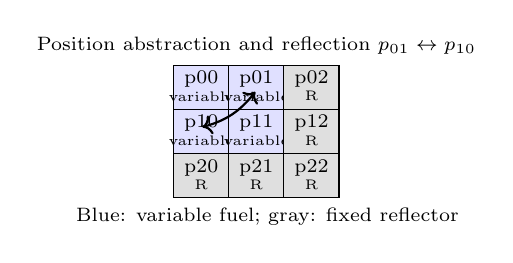
\begin{tikzpicture}[x=0.70cm,y=0.56cm]
\foreach \x/\y/\lab/\shadecolor in {
0/2/{p00}/blue!12,1/2/{p01}/blue!12,2/2/{p02}/gray!25,
0/1/{p10}/blue!12,1/1/{p11}/blue!12,2/1/{p12}/gray!25,
0/0/{p20}/gray!25,1/0/{p21}/gray!25,2/0/{p22}/gray!25}{
  \draw[fill=\shadecolor] (\x,\y) rectangle ++(1,1);
  \node[font=\scriptsize,align=center] at (\x+0.5,\y+0.68) {\lab};
  \node[font=\tiny,align=center] at (\x+0.5,\y+0.30) {\ifnum\x=2 R\else\ifnum\y=0 R\else variable\fi\fi};
}
\draw[<->,thick] (1.48,2.40) to[bend left=18] (0.52,1.60);
\node[font=\scriptsize,align=center] at (1.7,-0.43) {Blue: variable fuel; gray: fixed reflector};
\node[font=\scriptsize,align=center] at (1.5,3.45) {Position abstraction and reflection \(p_{01}\leftrightarrow p_{10}\)};
\end{tikzpicture}
\end{minipage}
\hfill
\begin{minipage}[t]{0.58\textwidth}
\centering
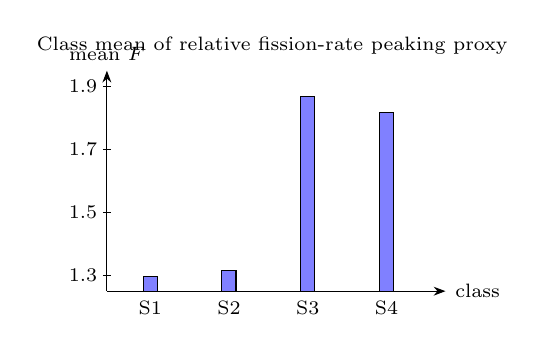
\begin{tikzpicture}[x=1.0cm,y=4.0cm]
\draw[-{Stealth[length=1.5mm]}] (0,0) -- (4.3,0) node[right,font=\scriptsize] {class};
\draw[-{Stealth[length=1.5mm]}] (0,0) -- (0,0.70) node[above,font=\scriptsize] {mean \(F\)};
\foreach \yt/\ylab in {0.05/1.3,0.25/1.5,0.45/1.7,0.65/1.9}{
 \draw (-0.05,\yt)--(0.05,\yt);
 \node[left,font=\scriptsize] at (0,\yt) {\ylab};
}
\foreach \x/\h/\lab in {0.55/0.045867/S1,1.55/0.066149/S2,2.55/0.617100/S3,3.55/0.566406/S4}{
 \draw[fill=blue!50,draw=black] (\x-0.09,0) rectangle (\x+0.09,\h);
 \node[font=\scriptsize,below] at (\x,0) {\lab};
}
\node[font=\scriptsize,align=center] at (2.1,0.78) {Class mean of relative fission-rate peaking proxy};
\end{tikzpicture}
\end{minipage}
\caption{(Left) Four variable fuel positions and five fixed reflector positions in the declared abstraction; diagonal reflection exchanges \(p_{01}\) and \(p_{10}\). (Right) Mean \(F\) by symmetry class. Class dispersion \(s_F\) is tabulated in Table~\ref{tab:classes}; it is not plotted because the class SDs are much smaller than the full vertical range.}
\label{fig:map_f}
\end{figure*}

\subsection{CB-PFR Status and Threshold Sensitivity}
For \(z=1\), the illustrative \(k_{\mathrm{eff}}\) bounds all fall within \([1.14,1.21]\), so \(V_k=0\) for all classes. Table~\ref{tab:screen} reports \(B_k^-\), \(B_k^+\), the upper operational bound \(B_F^+\), and aggregate normalized violation \(V_i\). Since \(V_k=0\) for all classes in this scenario, \(V_i=V_F=\max(0,B_F^+-F_{\max})/d_F\). Two classes pass (S1 and S2), represented by three layout labels; S3 and S4 fail. Since \(F_{\max}\) was selected retrospectively, this result demonstrates code behavior only.

\begin{table}[t]
\caption{Illustrative class-level CB-PFR screen: \(k\in[1.14,1.21]\), \(F_{\max}=1.35\), \(z=1\).}
\label{tab:screen}
\centering
\scriptsize
\setlength{\tabcolsep}{2.4pt}
\begin{tabular}{c c c r r l}
\toprule
Class & \(B_k^-\) & \(B_k^+\) & \(B_F^+\) & \(V_i\) & Status\\
\midrule
S1 & 1.143591 & 1.143781 & 1.296827 & 0.0000 & Pass\\
S2 & 1.156168 & 1.156358 & 1.317446 & 0.0000 & Pass\\
S3 & 1.186359 & 1.186639 & 1.868641 & 5.1864 & Fail\\
S4 & 1.204568 & 1.204762 & 1.817079 & 4.6708 & Fail\\
\bottomrule
\end{tabular}
\end{table}

Table~\ref{tab:sweep} reports counts as \emph{label strings / symmetry classes}; for example, S1 contributes two label strings but one physical class. The \(z=0\) and \(z=1\) counts coincide across this tested grid; \(z=2\) changes the count only at \(F_{\max}=1.87\). The passing count is therefore dependent on the retrospective cutoff, which is not independently justified as a physical limit.

\begin{table}[t]
\caption{Retrospective sensitivity sweep: passing label strings / symmetry classes.}
\label{tab:sweep}
\centering
\scriptsize
\setlength{\tabcolsep}{3pt}
\begin{tabular}{c c c c}
\toprule
\(F_{\max}\) & \(z=0\) & \(z=1\) & \(z=2\)\\
\midrule
1.30 & 2 / 1 & 2 / 1 & 2 / 1\\
1.32 & 3 / 2 & 3 / 2 & 3 / 2\\
1.35 & 3 / 2 & 3 / 2 & 3 / 2\\
1.80 & 3 / 2 & 3 / 2 & 3 / 2\\
1.82 & 5 / 3 & 5 / 3 & 5 / 3\\
1.87 & 6 / 4 & 6 / 4 & 5 / 3\\
1.90 & 6 / 4 & 6 / 4 & 6 / 4\\
\bottomrule
\end{tabular}
\end{table}

\subsection{UMMU Repeatability and Protocol Audit}
Table~\ref{tab:ummu} compares two archived three-seed UMMU run sets. Both used 7,000 total batches, 10,000 particles per batch, the same multigroup cross-section hash, unique random seeds, and passing raw HDF5/group-structure audits; the inactive-batch setting differs. The mean shifts from $k_{\mathrm{ref}}=1.18655$ are expressed in absolute pcm as $(\bar{k}-k_{\mathrm{ref}})\times10^5$. The project reference uncertainty is $u_{\mathrm{ref}}=9.5\times10^{-5}$ in absolute $k_{\mathrm{eff}}$ units (9.5 pcm); it is not a relative uncertainty or an official benchmark tolerance.

For a descriptive combined-uncertainty score only, we use
\[
u_{\mathrm{run}}=\frac{\max(s_{\mathrm{between}},s_{\mathrm{within}})}{\sqrt{n}},\qquad
z_{\mathrm{comb}}=\frac{\bar{k}-k_{\mathrm{ref}}}
{\sqrt{u_{\mathrm{ref}}^2+u_{\mathrm{run}}^2}},
\]
where $s_{\mathrm{between}}$ is the sample SD of run means and $s_{\mathrm{within}}$ is the pooled within-run reported SD. This conservative operational convention yields $z_{\mathrm{comb}}=-0.434$ for the 500-inactive set and $-0.698$ for the 100-inactive set. It is a descriptive project calculation, not an acceptance criterion or evidence of benchmark validation.

\begin{table*}[t]
\caption{Separate UMMU run protocols and repeatability summaries.}
\label{tab:ummu}
\centering
\small
\setlength{\tabcolsep}{5pt}
\begin{tabular}{l r r r r r}
\toprule
Protocol & Inactive batches & Mean $k_{\mathrm{eff}}$ & $\Delta k$ (pcm) & Between-run SD (pcm) & Pooled within-run SD (pcm)\\
\midrule
A & 500 & 1.18649321 & $-5.68$ & 15.57 & 9.58\\
B & 100 & 1.18647358 & $-7.64$ & 0.77 & 9.45\\
\bottomrule
\end{tabular}
\end{table*}

The two protocol summaries must not be merged: between-run SD is about 1.63 times the pooled within-run SD for Protocol A but only 0.081 times that SD for Protocol B. The latter is a pronounced under-dispersion relative to the run-level uncertainty estimates and requires investigation rather than interpretation as unusually strong repeatability. Active-trace first-to-last-quartile $k$-generation shifts are $+24.0$ to $+65.1$ pcm for Protocol A and $-16.1$ to $+23.5$ pcm for Protocol B. The corresponding entropy shifts are $-0.00195$ to $-0.00007$ and $-1.456$ to $-0.475$, respectively; the 100-inactive logs also recorded repeated source sites outside the entropy mesh. These traces do not certify source convergence. Neither protocol is treated as a validated canonical estimate; model/tally review and convergence investigation remain necessary.

\section{Discussion}
The results illustrate three distinct issues. First, the composition-only QUBO enforces the material count but ties all feasible layouts by construction. Second, CB-PFR can make operational screening decisions auditable, but a threshold selected after observing the study data supports retrospective sensitivity analysis only. Third, candidate ties must be preserved at the symmetry-class level when the model and data do not distinguish mirror orientations. The secondary proxy \(F\) separates the four class means descriptively, but this small enumerated case does not demonstrate comparative benefit over a baseline or the value of running an optimizer before simulation.

The paper does not claim that the selected proxy is an engineering acceptance criterion. A stronger confirmatory study would require physical limits justified independently of this campaign, a prospectively specified analysis, independent model/tally review, and an adequate comparison against simple methods. A larger candidate space and a meaningful physics-sensitive pre-physics objective would be required to evaluate claims about optimizer utility. Constraint-handling methods and simulation ranking-and-selection have established literature \cite{deb2000,kimnelson2006}. For uncertainty terminology, the paper distinguishes within-run Monte Carlo standard uncertainties from observed between-run dispersion, consistent with measurement-uncertainty guidance \cite{taylor1994}. Other C5G7 deterministic transport studies provide methodological context but are not treated as direct performance baselines for CB-PFR \cite{song2020}. The contribution is the explicit software workflow and its evidence-bounded audit, not priority for feasibility-first ranking.

\section{Conclusion}
This paper reports an exploratory, evidence-audited CB-PFR workflow on six enumerated C5G7-derived fuel layouts. The composition QUBO assigns zero energy to each feasible layout; diagonal-reflection symmetry reduces six labels to four classes. Under a retrospective illustrative screen, two classes pass and two fail, while the sensitivity table makes threshold dependence explicit. The separate UMMU run sets give absolute reference differences of \(-5.68\) pcm and \(-7.64\) pcm under 500- and 100-inactive-batch protocols, respectively. Their repeatability diagnostics differ materially, and neither establishes benchmark acceptance. The evidence supports workflow traceability and transparent handling of ties, not physical optimality, calibrated confidence coverage, full validation, or method superiority.

\section*{Software and Data Availability}
The accompanying anonymous-review supplement contains the 18-run six-layout table, six UMMU run-level records with statepoint hashes, a two-protocol summary and source-trace diagnostics, and the scripts needed to reproduce the reported aggregation rules. The project identity and permanent public release are withheld from this double-blind manuscript; no DOI or public release is claimed in this review version.

\bibliographystyle{IEEEtran}
\bibliography{references}
\end{document}
